\documentclass[letterpaper,12pt,fleqn]{article}
\usepackage{matharticle}
\usepackage{siunitx}
\pagestyle{plain}
\begin{document}

\begin{center}
\Large Math-1003b Homework \#7 Solutions
\end{center}

\vspace{0.5in}

\underline{Reading}

\bigskip

\begin{itemize}
\item Section 9.1 and 9.2
\end{itemize}

\bigskip

\underline{Problems}

\bigskip

\begin{enumerate}
\item Let $A=\{x\in\R\mid -1\le x<3\}$ and $B=\{x\in\R\mid x<\frac{1}{2}\}$.
  \begin{enumerate}
  \item Graph $A$ and express in interval notation.

    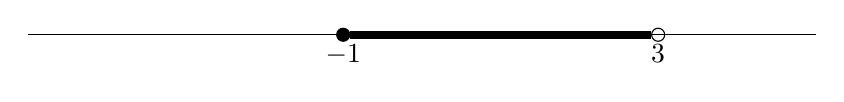
\begin{tikzpicture}
      \draw (-5,0) -- (5,0);
      \node [circle,draw,fill,scale=0.5] (a) at (-1,0) {};
      \node [below] at (a) {$-1$};
      \node [circle,draw,scale=0.5] (b) at (3,0) {};
      \node [below] at (b) {$3$};
      \draw [line width=1mm] (a) to (b);
    \end{tikzpicture}
    $A=[-1,3)$
    
  \item Graph $B$ and express in interval notation.

    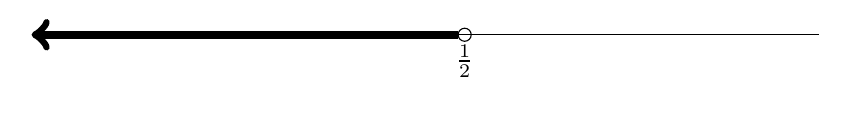
\begin{tikzpicture}
      \draw (-5,0) -- (5,0);
      \node [circle,draw,scale=0.5] (a) at ({1/2},0) {};
      \node [below] at (a) {$\frac{1}{2}$};
      \draw [line width=1mm,->] (a) to (-5,0);
    \end{tikzpicture}
    $B=(-\infty,\frac{1}{2})$
    
  \item Graph $A\cup B$ and express in interval notation.

    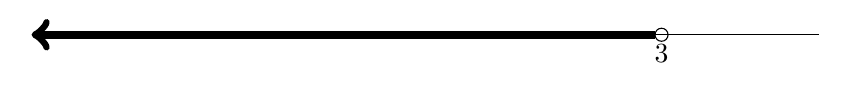
\begin{tikzpicture}
      \draw (-5,0) -- (5,0);
      \node [circle,draw,scale=0.5] (a) at (3,0) {};
      \node [below] at (a) {$3$};
      \draw [line width=1mm,->] (a) to (-5,0);
    \end{tikzpicture}
    $A\cup B=(-\infty,3)$    

  \item Graph $A\cap B$ and express in interval notation.
    
    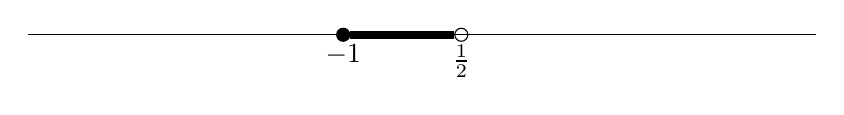
\begin{tikzpicture}
      \draw (-5,0) -- (5,0);
      \node [circle,draw,fill,scale=0.5] (a) at (-1,0) {};
      \node [below] at (a) {$-1$};
      \node [circle,draw,scale=0.5] (b) at ({1/2},0) {};
      \node [below] at (b) {$\frac{1}{2}$};
      \draw [line width=1mm] (a) to (b);
    \end{tikzpicture}
    $A\cap B=[-1,\frac{1}{2})$

  \end{enumerate}

\item Let $f(x)=3-2x$
  \begin{enumerate}
  \item Solve for $x$:
    \[5<f(x)\le 9\]
    and express the answer in interval notation.

    Since this is a compound inequality (and/intersection) we can solve simultaneously:
    \[\begin{array}{l}
      5<3-2x\le 9 \\
      2<-2x\le 6 \\
      -1>x\ge -3 \\
      -3\le x< -1
    \end{array}\]
    $x\in[-3,-1)$
    
  \item Solve for $x$:
    \[5<f(x)\ \mbox{or}\ f(x)>9\]
    and express the answer in interval notation.

    Solve each inequality separately:

    \begin{minipage}{3in}
      $3-2x>5$ \\
      $-2x>2$ \\
      $x<-1$
    \end{minipage}
    \begin{minipage}{3in}
      $3-2x>9$ \\
      $-2x>6$ \\
      $x<-3$
    \end{minipage}
  \end{enumerate}

  Now graph each one and take the union (or):
  
    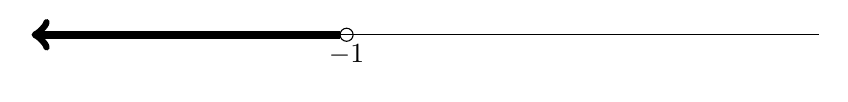
\begin{tikzpicture}
      \draw (-5,0) -- (5,0);
      \node [circle,draw,scale=0.5] (a) at (-1,0) {};
      \node [below] at (a) {$-1$};
      \draw [line width=1mm,<-] (-5,0) to (a);
    \end{tikzpicture}
    $A=(-\infty,-1)$
    
    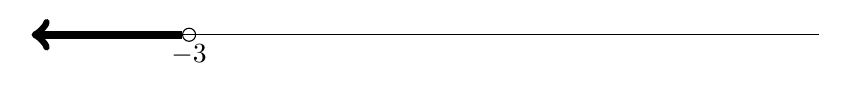
\begin{tikzpicture}
      \draw (-5,0) -- (5,0);
      \node [circle,draw,scale=0.5] (b) at (-3,0) {};
      \node [below] at (b) {$-3$};
      \draw [line width=1mm,<-] (-5,0) to (b);
    \end{tikzpicture}
    $B=(-\infty,-3)$
    
    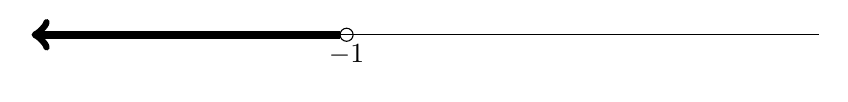
\begin{tikzpicture}
      \draw (-5,0) -- (5,0);
      \node [circle,draw,scale=0.5] (a) at (-1,0) {};
      \node [below] at (a) {$-1$};
      \draw [line width=1mm,<-] (-5,0) to (a);
    \end{tikzpicture}
    $A\cup B=(-\infty,-1)$

    Note that $A$ is a superset of $B$, so the union will be the superset.
\end{enumerate}

\end{document}
